\documentclass[10pt]{beamer}

\usetheme{Madrid}
\usecolortheme{default}

% Base packages
%\usepackage{helvet}
\usepackage{amsmath,amssymb,amsthm,mathtools,subcaption}
\usepackage{tikz,pgfplots,tabularx,booktabs}
\usetikzlibrary{arrows.meta, positioning, quotes}

\usepackage{xcolor}

%\usepackage[cache=false]{minted}
%\renewcommand{\theFancyVerbLine}{\sffamily\textcolor[rgb]{0.5,0.5,1.0}{\scriptsize\oldstylenums{\arabic{FancyVerbLine}}}}
%\definecolor{bg}{rgb}{.95,.95,.95}

% Font settings
\renewcommand{\familydefault}{\sfdefault}

% TikZ libraries
\usetikzlibrary{calc,positioning,backgrounds,decorations.pathreplacing}
\pgfplotsset{compat=1.14}

% Colors
\definecolor{deepblue}{RGB}{42,39,155}
\definecolor{lightpink}{RGB}{255,240,240}
\definecolor{lightgreen}{RGB}{240,255,240}
\definecolor{lightyellow}{RGB}{255,255,240}
\definecolor{codegray}{RGB}{245,245,245}
\definecolor{codegreen}{rgb}{0,0.6,0}
\definecolor{codepurple}{rgb}{0.58,0,0.82}

% Beamer settings
\setbeamercolor{title}{fg=white,bg=deepblue}
\setbeamercolor{frametitle}{fg=white,bg=deepblue}
\setbeamercolor{section in head/foot}{fg=white,bg=deepblue}

\setbeamertemplate{footline}[text line]{%
  \parbox{\linewidth}{\vspace*{-8pt}
  %\hfill\href{https://github.com/chang-ye-tu/fin}{https://github.com/chang-ye-tu/fin}
    \hfill
   \insertframenumber~/ \inserttotalframenumber}}
\setbeamertemplate{navigation symbols}{}%[only frame symbol]

\definecolor{foo}{rgb}{.2,.2,.7}
\AtBeginSection[]{
  \begin{frame}
  \vfill
  \centering
  \begin{beamercolorbox}[sep=8pt,center,shadow=true,rounded=true]{section page}
    \usebeamerfont{title}%
    {\color{foo} \insertsectionhead}\par%
  \end{beamercolorbox}
  \vfill
  \end{frame}
}

% https://tex.stackexchange.com/questions/30423/bibliography-in-beamer
\setbeamertemplate{bibliography entry title}{}
\setbeamertemplate{bibliography entry location}{}
\setbeamertemplate{bibliography entry note}{}

\DeclareMathOperator\prb{\mathsf{P}}
\DeclareMathOperator\expc{\mathsf{E}}
\DeclareMathOperator\var{var}
\DeclareMathOperator\cov{cov}
\DeclareMathOperator\cor{corr}
\DeclareMathOperator*{\argmax}{\arg\!\max}
\DeclareMathOperator*{\argmin}{\arg\!\min}
\DeclareMathOperator\corr{corr}
\DeclareMathOperator\rk{rank}
\DeclareMathOperator\sgn{sgn}
\DeclareMathOperator{\tr}{tr}

% Blackboard bold
\renewcommand{\AA}{\mathbb A}
\newcommand{\CC}{\mathbb C}
\newcommand{\DD}{\mathbb D}
\newcommand{\EE}{\mathbb E}
\newcommand{\FF}{\mathbb F}
\newcommand{\HH}{\mathbb H}
\newcommand{\KK}{\mathbb K}
\newcommand{\NN}{\mathbb N}
\newcommand{\PP}{\mathbb P}
\newcommand{\QQ}{\mathbb Q}
\newcommand{\RR}{\mathbb R}
\newcommand{\UU}{\mathbb U}
\newcommand{\ZZ}{\mathbb Z}

\newcommand{\ie}{\;\Longrightarrow\;}
\newcommand{\ifff}{\;\Longleftrightarrow\;}
\newcommand{\ds}{\displaystyle}

\title{Introduction to Financial Models \\ Lecture 04: Surprises \& Paradoxes III}
\author{}
\date{}

\begin{document}

\begin{frame}
\titlepage
\end{frame}

%\subsection*{Outline}
%\begin{frame}
%  \tableofcontents
%\end{frame}

\begin{frame}{St. Petersburg Paradox}
  \begin{itemize}[<+->]
    \item Proposed by Nicolas Bernoulli in 1713, analyzed by Daniel Bernoulli in 1738
    \item The game:
      \begin{itemize}
        \item Flip a fair coin until it shows heads
        \item If heads appears on the first flip, win \$2
        \item If heads appears on the second flip, win \$4
        \item If heads appears on the third flip, win \$8
        \item In general, if heads appears on the $n$-th flip, win \$$2^n$
      \end{itemize}
    \item The expected value calculation:
      \begin{align*}
        \expc{X} = \sum_{n=1}^{\infty} 2^n \cdot \prb(\text{heads on flip } n) = \sum_{n=1}^{\infty} 2^n \cdot \frac{1}{2^n} = \sum_{n=1}^{\infty} 1 = \infty
      \end{align*}
    \item Note that $\sum_{k=1}^n 2^k = 2^{n + 1} - 2$
    \item The paradox: The game has infinite expected value, but most people would only pay a small amount to play
    \item If people maximize expected value, they should be willing to pay any finite amount to play
  \end{itemize}
\end{frame}

\begin{frame}{Early Solutions to the Paradox}
  \begin{itemize}[<+->]
    \item Practical resolution: No casino has infinite resources
      \begin{itemize}
        \item With a capped maximum payout of $M$, $\expc{X} \approx \lfloor \log_2 M \rfloor$
        \item For $M = 2^{20} \approx$ \$1 million, $\expc{X} \approx$ \$20
      \end{itemize}
    \item Daniel Bernoulli's insight (1738): People value money differently
      \begin{itemize}
        \item ``The value of an item must not be based on its price, but rather on the utility it yields''
        \item Proposed logarithmic utility function: $U(w) = \log(w)$
        \item Diminishing marginal utility: Each extra dollar adds less utility
      \end{itemize}
    \item Gabriel Cramer (1728) suggested: $U(w) = \sqrt{w}$ 
    \item Note that if $\forall\,|x| < 1$, $f(x) = \sum_{n=0}^\infty x^n = \frac{1}{1 - x}$, then $\sum_{n=1}^\infty nx^n = xf'(x) = \frac{x}{(1 - x)^2}$.
    \item With logarithmic utility, expected utility is finite:
      \begin{align*}
        \expc{U(X)} = \sum_{n=1}^{\infty} \log(2^n) \cdot \frac{1}{2^n} = \sum_{n=1}^{\infty} \frac{n \log(2)}{2^n} = 2\log(2) < \infty
      \end{align*}
    \item This amounts to $\expc{U(X)} \approx$ \$1.39, explaining why people would only pay a small amount
  \end{itemize}
\end{frame}

\begin{frame}{The Expected Utility Hypothesis}
  \begin{block}{Mathematical Formulation}
    The agent prefers the r.v. $X$ to r.v. $Y$ if and only if $\expc U(X) > \expc U(Y)$, where $U:\RR\mapsto\RR$ is the agent's utility function.
  \end{block}
  \vspace{3mm}
  \onslide<+-> 
  \begin{itemize}[<+->]
    \item Expected utility theory attempts to explain how people make decisions under uncertainty
    \item It seeks to address paradoxes like St. Petersburg by incorporating risk preferences
    \item Key insight: people care about the utility of outcomes, not just monetary values
    \item Decision-making is based on:
      \begin{enumerate}
        \item Probabilities of different outcomes
        \item Subjective valuation (utility) of those outcomes
      \end{enumerate}
  \end{itemize}
\end{frame}

\begin{frame}{Properties of Utility Functions}
  \begin{itemize}[<+->]
    \item Three common assumptions about utility functions:
      \begin{itemize}
        \item \textbf{More is better}: $U'(w) > 0$ (monotonically increasing)
        \item \textbf{Risk aversion}: $U''(w) < 0$ (concave function)
        \item \textbf{Decreasing absolute risk aversion}: $-\frac{U''(w)}{U'(w)}$ decreases as $w$ increases
      \end{itemize}
    \item Commonly used utility functions:
      \begin{itemize}
        \item Logarithmic: $U(w) = \log(w)$
        \item Power utility: $U(w) = \frac{w^{1-\gamma} - 1}{1-\gamma}$ for $\gamma > 0, \gamma \neq 1$
        \item Exponential utility: $U(w) = -e^{-\gamma w}$ for $\gamma > 0$
        \item Quadratic utility: $U(w) = w - \frac{\gamma}{2}w^2$ for $w < \frac{1}{\gamma}$
      \end{itemize}
    \item The parameter $\gamma$ reflects the degree of risk aversion
    \item For power utility, $\gamma = 1$ corresponds to logarithmic utility (by L'Hôpital's rule)
  \end{itemize}
\end{frame}

\begin{frame}{Risk Aversion and Risk Premium I}
  \begin{itemize}[<+->]
    \item Risk Aversion
      \begin{itemize}
        \item The \textbf{risk aversion} is the preference for a certain amount over a gamble with the same expected value
        \item Example: Preferring \$50 with certainty over a 50\% chance of \$100 (and 50\% chance of \$0)
        \item Mathematically represented by a concave utility function: $U''(w) < 0$
      \end{itemize}
    \item Risk Premium 
      \begin{itemize}
        \item Let $\widetilde{X}$ be a random variable with $\expc{\widetilde{X}} = 0$ (a fair gamble)
        \item A risk-averse person would pay to avoid this gamble
        \item The \textbf{risk premium} $\pi$ is the maximum amount they would pay:
          \begin{align}\label{eq:risk_premium}
            U(w - \pi) = \expc{U(w + \widetilde{X})}
          \end{align}
      \end{itemize}
  \end{itemize}
\end{frame}

\begin{frame}{Risk Aversion and Risk Premium II}
  \begin{itemize}[<+->]
    \item For small risks, we can use Taylor expansion 
      \begin{align*}
        U(w + \widetilde{X}) &\approx U(w) + U'(w)\widetilde{X} + \frac{1}{2}U''(w)\widetilde{X}^2
      \end{align*}
    \item By $\expc{\widetilde{X}} = 0$ and $\var{\widetilde{X}} = \expc{\widetilde{X}^2} - (\expc{\widetilde{X}})^2 = \expc{\widetilde{X}^2}$, 
      \begin{align*}
        \expc{U(w + \widetilde{X})} &\approx U(w) + U'(w)\expc{\widetilde{X}} + \frac{1}{2}U''(w)\expc{\widetilde{X}^2} = U(w) + \frac{1}{2}U''(w)\var{\widetilde{X}}
      \end{align*}
    \item Similarly, for small premium, one can use Taylor expansion 
      \begin{align*}
        U(w - \pi) \approx U(w) - \pi U'(w)
      \end{align*}
    \item Substitute into the risk premium formula \eqref{eq:risk_premium} $U(w - \pi) = \expc{U(w + \widetilde{X})}$,
      \begin{align*}
        U(w) - \pi U'(w) = U(w) + \frac{1}{2}U''(w)\var{\widetilde{X}} \ie \pi = \frac{1}{2}\left(-\frac{U''(w)}{U'(w)}\right)\var{\widetilde{X}}
      \end{align*}
  \end{itemize}
\end{frame}

\begin{frame}{Risk Aversion and Risk Premium - III}
    \begin{itemize}[<+->]
      \item The term $-\frac{U''(w)}{U'(w)}$ is the coefficient of absolute risk aversion (ARA)
        \begin{itemize}
          \item Measures risk aversion in absolute dollar terms
          \item Logarithmic utility: ARA = $\frac{1}{w}$ (decreasing with wealth)
          \item Power utility: ARA = $\frac{\gamma}{w}$ (decreasing with wealth)
          \item Exponential utility: ARA = $\gamma$ (constant regardless of wealth)
        \end{itemize}
      \item The term $-\frac{U''(w)}{U'(w)} \cdot w$ is the coefficient of relative risk aversion (RRA)
        \begin{itemize}
          \item Measures risk aversion relative to wealth level
          \item Logarithmic utility: RRA = 1 (constant)
          \item Power utility: RRA = $\gamma$ (constant)
          \item Exponential utility: RRA = $\gamma w$ (increasing with wealth)
        \end{itemize}
    \end{itemize}
\end{frame}

\begin{frame}{Axiomatic Foundation of Expected Utility}
  \begin{itemize}[<+->]
    \item John von Neumann and Oskar Morgenstern (1947) provided axioms for expected utility
    \item Four key axioms:
      \begin{itemize}
        \item \textbf{Completeness}: For any lotteries $L_1$ and $L_2$, either $L_1 \succeq L_2$ or $L_2 \succeq L_1$ or both
        \item \textbf{Transitivity}: If $L_1 \succeq L_2$ and $L_2 \succeq L_3$, then $L_1 \succeq L_3$
        \item \textbf{Continuity}: If $L_1 \succeq L_2 \succeq L_3$, then there exists a probability $p \in [0, 1]$ such that $L_2 \sim p L_1 + (1-p) L_3$
        \item \textbf{Independence}: For any lotteries $L_1$, $L_2$, $L_3$ and any probability $p \in (0, 1]$, $L_1 \succeq L_2$ if and only if $p L_1 + (1-p) L_3 \succeq p L_2 + (1-p) L_3$
      \end{itemize}
    \item These axioms lead to the expected utility representation:
      \begin{align*}
        L_1 \succeq L_2 \iff \expc_{L_1}[U(x)] \geqslant \expc_{L_2}[U(x)]
      \end{align*}
    \item The independence axiom is particularly important and controversial
      \begin{itemize}
        \item It states that preferences between lotteries should not be affected by mixing them with a third lottery
        \item This axiom is violated in several famous paradoxes
      \end{itemize}
  \end{itemize}
\end{frame}

\begin{frame}{Allais Paradox}
  \begin{itemize}[<+->]\setlength\itemsep{0em}
    \item Game A
      \begin{align*}
        X = \begin{cases}101 & \text{prob. } 0.33\\100 & \text{prob. } 0.66\\ 0 & \text{prob. } 0.01 \end{cases} \qquad
        Y = 100 \;\text{ with prob. } 1
      \end{align*}
      \onslide<+->
      Mostly prefer $Y$ to $X$: from the Expected Utility Hypothesis 
      \onslide<+->
      \begin{multline}
        U(100) > 0.33\cdot U(101) + 0.66\cdot U(100) + 0.01\cdot U(0)\\ \ie 0.34\cdot U(100) > 0.33\cdot U(101) + 0.01\cdot U(0)
      \end{multline}
    \item Game B 
      \begin{align*}
        X = \begin{cases}100 & \text{prob. } 0.34\\ 0 & \text{prob. } 0.66 \end{cases} \qquad
        Y = \begin{cases}101 & \text{prob. } 0.33\\ 0 & \text{prob. } 0.67 \end{cases}
      \end{align*}
      \onslide<+->
      Mostly prefer $Y$ to $X$: from the Expected Utility Hypothesis 
      \onslide<+->
      \begin{multline}
        0.33\cdot U(101) + 0.67\cdot U(0) > 0.34\cdot U(100) + 0.66\cdot U(0)\\ \ie 0.33\cdot U(101) + 0.01\cdot U(0) > 0.34\cdot U(100)
      \end{multline}
  \end{itemize}
\end{frame}

\begin{frame}{Ellsberg Paradox}
  \begin{itemize}[<+->]
    \item Given an urn with $30$ balls of colors red, yellow, and black
    \item There are $10$ red balls; total $20$ yellow / black balls, but the number of each type unknown
    \item The agent estimates the probability of drawing yellow as $p$ where $0 < p < \frac{2}{3}$
    \item A single ball is drawn from the urn
  \end{itemize}
\end{frame}

\begin{frame}{Ellsberg Paradox (Cont'd)}
  \begin{itemize}[<+->]\setlength\itemsep{0em}
    \item Game A  
      \begin{align*}
        X = \begin{cases}100 & \text{if red}\\0 & \text{if yellow or black}\end{cases} \qquad
        Y = \begin{cases}100 & \text{if yellow}\\0 & \text{if red or black}\end{cases} \qquad
      \end{align*}
      \onslide<+->
      Mostly prefer $X$ to $Y$: from the Expected Utility Hypothesis 
      \onslide<+->
      \begin{multline}
        \frac{1}{3}\cdot U(100) + \frac{2}{3}\cdot U(0) > p\cdot U(100) + (1 - p)\cdot U(0) \\ \ie\big(\frac{1}{3} - p\big)\cdot U(100) > \big(\frac{1}{3} - p\big)\cdot U(0)
      \end{multline}
    \item Game B 
      \begin{align*}
        X = \begin{cases}100 & \text{if red or black}\\ 0 & \text{if yellow}\end{cases} \qquad
        Y = \begin{cases}100 & \text{if yellow or black}\\ 0 & \text{if red}\end{cases}
      \end{align*}
      \onslide<+->
      Mostly prefer $Y$ to $X$: from the Expected Utility Hypothesis 
      \onslide<+->
      \begin{multline}
        \frac{2}{3}\cdot U(100) + \frac{1}{3}\cdot U(0) > (1 - p)\cdot U(100) + p\cdot U(0) \\ \ie\big(\frac{1}{3} - p\big)\cdot U(0) > \big(\frac{1}{3} - p\big)\cdot U(100)
      \end{multline}
  \end{itemize}
\end{frame}

\begin{frame}{Limitations of Expected Utility Theory}
  \begin{itemize}[<+->]
    \item The Allais and Ellsberg paradoxes highlight systematic violations of expected utility theory
    \item Key limitations:
      \begin{itemize}
        \item Violation of the independence axiom
        \item Inability to account for ambiguity aversion
        \item Failure to explain reference-dependent preferences
        \item Inconsistent treatment of gains versus losses
      \end{itemize}
    \item These limitations led Kahneman and Tversky to develop alternative models
    \item Their research culminated in Prospect Theory (1979) and Cumulative Prospect Theory (1992)
    \item Won the Nobel Prize in Economics in 2002 (Kahneman; Tversky had passed away)
  \end{itemize}
\end{frame}

\begin{frame}{Prospect Theory -- Key Innovations}
  \begin{itemize}[<+->]
    \item Developed by Daniel Kahneman and Amos Tversky (1979)
    \item Four major innovations over expected utility theory:
      \begin{itemize}
        \item \textbf{Reference dependence}: Outcomes evaluated as gains or losses relative to a reference point
        \item \textbf{Loss aversion}: Losses hurt more than equivalent gains feel good
        \item \textbf{Diminishing sensitivity}: Marginal value decreases with distance from reference point
        \item \textbf{Probability weighting}: People overweight small probabilities and underweight large ones
      \end{itemize}
    \item Mathematical representation: 
      \begin{align*}
        V(\text{prospect}) = \sum_{i} \pi(p_i) \cdot v(x_i)
      \end{align*}
      where $v(x)$ is the value function and $\pi(p)$ is the probability weighting function
  \end{itemize}
\end{frame}

\begin{frame}{The Value Function}
  \begin{columns}
    \begin{column}{0.55\textwidth}
      \begin{itemize}[<+->]
        \item The value function $v(x)$ is:
          \begin{itemize}
            \item Defined on gains and losses (deviations from reference point)
            \item Steeper for losses than for gains (loss aversion)
            \item Concave for gains (risk aversion)
            \item Convex for losses (risk seeking)
          \end{itemize}
        \item Typical parametrization:
          \begin{align*}
            v(x) = 
            \begin{cases}
              x^{\alpha} & \text{if } x \geq 0 \\
              -\lambda(-x)^{\beta} & \text{if } x < 0
            \end{cases}
          \end{align*}
        \item Parameter values:
          \begin{itemize}
            \item $\alpha, \beta \approx 0.88$ (diminishing sensitivity)
            \item $\lambda \approx 2.25$ (loss aversion coefficient)
          \end{itemize}
      \end{itemize}
    \end{column}
    \begin{column}{0.45\textwidth}
      \onslide<+->
      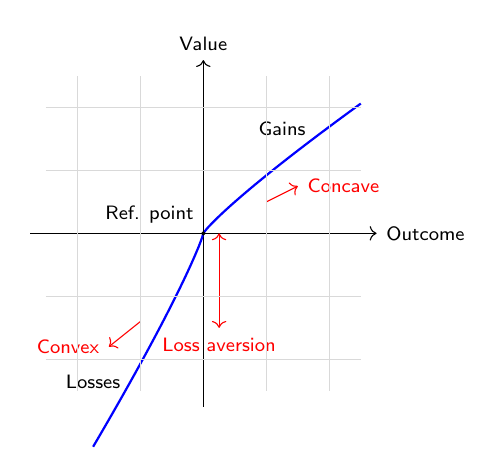
\begin{tikzpicture}[scale=0.4]
        \draw[->] (-5.5,0) -- (5.5,0) node[right, font=\scriptsize] {Outcome};
        \draw[->] (0,-5.5) -- (0,5.5) node[above, font=\scriptsize] {Value};
        
        % Value function
        \draw[domain=0:5, blue, thick, samples=100] plot (\x, {pow(\x, 0.88)});
        \draw[domain=-3.5:0, blue, thick, samples=100] plot (\x, {-2.25*pow(-\x, 0.88)});
        
        % Reference point
        \filldraw (0,0) circle (1.5pt) node[above left, font=\scriptsize] {Ref. point};
        
        % Labels
        \node[above, font=\scriptsize] at (2.5,2.8) {Gains};
        \node[below, font=\scriptsize] at (-3.5,-4.2) {Losses};
        
        % Annotations
        \draw[->, red, thin] (2,1.) -- (3,1.5) node[right, font=\scriptsize] {Concave};
        \draw[->, red, thin] (-2,-2.8) -- (-3,-3.6) node[left, font=\scriptsize] {Convex};
        \draw[<->, red, thin] (0.5,0.) -- (0.5,-3) node[below, font=\scriptsize] {Loss aversion};
        
        % Grid lines (faint)
        \foreach \x in {-4,-2,2,4}
          \draw[gray!30] (\x,-5) -- (\x,5);
        \foreach \y in {-4,-2,2,4}
          \draw[gray!30] (-5,\y) -- (5,\y);
      \end{tikzpicture}
    \end{column}
  \end{columns}
\end{frame}

\begin{frame}{Probability Weighting Function}
  \begin{columns}
    \begin{column}{0.5\textwidth}
      \begin{itemize}[<+->]
        \item People do not process probabilities linearly
        \item Probability weighting function $\pi(p)$:
          \begin{itemize}
            \item Overweights small probabilities: $\pi(p) > p$ for small $p$
            \item Underweights large probabilities: $\pi(p) < p$ for large $p$
            \item Fixed points at $p = 0$ and $p = 1$
            \item Inverse S-shaped curve
          \end{itemize}
        \item Tversky and Kahneman's (1992) formulation:
          \begin{align*}
            \pi(p) = \frac{p^{\gamma}}{(p^{\gamma} + (1-p)^{\gamma})^{1/\gamma}}
          \end{align*}
        \item Typical parameter value: $\gamma \approx 0.65$
      \end{itemize}
    \end{column}
    \begin{column}{0.5\textwidth}
      \onslide<+->
      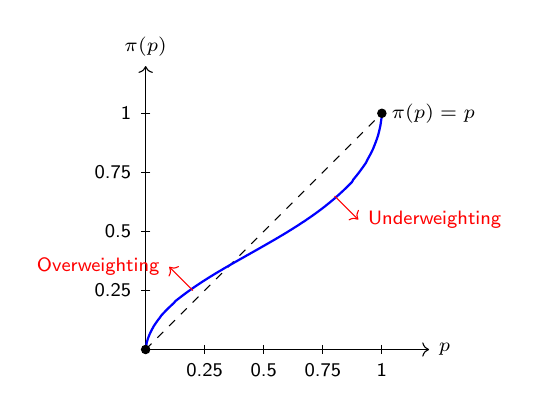
\begin{tikzpicture}[scale=3]
        \draw[->] (0,0) -- (1.2,0) node[right, font=\scriptsize] {$p$};
        \draw[->] (0,0) -- (0,1.2) node[above, font=\scriptsize] {$\pi(p)$};
        
        % Linear probability
        \draw[domain=0:1, dashed] plot (\x, \x) node[right, font=\scriptsize] {$\pi(p) = p$};
        
        % Weighting function - correct implementation of the Tversky-Kahneman formula
        \draw[domain=0.0:1.0, blue, thick, samples=200] plot (\x, {(\x^0.65)/((\x^0.65 + (1-\x)^0.65)^(1/0.65))});
        
        % Points
        \filldraw (0,0) circle (0.5pt);
        \filldraw (1,1) circle (0.5pt);
        
        % Grid lines
        \foreach \x in {0.25,0.5,0.75,1}
          \draw (\x,0.02) -- (\x,-0.02) node[below, font=\scriptsize] {\x};
        \foreach \y in {0.25,0.5,0.75,1}
          \draw (0.02,\y) -- (-0.02,\y) node[left, font=\scriptsize] {\y};
        
        % Annotations
        \draw[->, red, thin] (0.2,0.25) -- (0.1,0.35) node[left, font=\scriptsize] {Overweighting};
        \draw[->, red, thin] (0.8,0.65) -- (0.9,0.55) node[right, font=\scriptsize] {Underweighting};
      \end{tikzpicture}
    \end{column}
  \end{columns}
\end{frame}

\begin{frame}{Key Findings: Asian Disease Problem}
  \begin{itemize}[<+->]
    \item Asian Disease Problem (Tversky \& Kahneman, 1981)
      \begin{itemize}
        \item One of the most famous demonstrations of framing effects
        \item Scenario: "Imagine the U.S. is preparing for an outbreak of an unusual Asian disease expected to kill 600 people. Two alternative programs to combat the disease have been proposed."
        \item \textbf{Gain frame} (first group of participants):
          \begin{itemize}
            \item Program A: "200 people will be saved" (certainty)
            \item Program B: "1/3 probability 600 people will be saved, and 2/3 probability no people will be saved" (risk)
            \item Result: 72\% chose Program A (risk-averse preference)
          \end{itemize}
        \item \textbf{Loss frame} (second group of participants):
          \begin{itemize}
            \item Program C: "400 people will die" (certainty)
            \item Program D: "1/3 probability nobody will die, and 2/3 probability 600 people will die" (risk)
            \item Result: 78\% chose Program D (risk-seeking preference)
          \end{itemize}
        \item Programs A and C are identical in outcomes, as are B and D
        \item The shift in preferences demonstrates that people are risk-averse for gains (saving lives) but risk-seeking for losses (avoiding deaths)
      \end{itemize}
  \end{itemize}
\end{frame}

\begin{frame}{Key Findings: The Reflection Effect}
  \begin{itemize}[<+->]
    \item The Reflection Effect (Kahneman \& Tversky, 1979)
      \begin{itemize}
        \item Core finding: Risk preferences "reflect" (reverse) when prospects are transformed from gains to losses
        \item Positive prospects (gains): People generally risk-averse
        \item Negative prospects (losses): People generally risk-seeking
      \end{itemize}
    \item Experimental evidence:
      \begin{itemize}
        \item Study participants chose between pairs of prospects
        \item \textbf{Problem 3} (N=95):
          \begin{align*}
            &\text{A: } (4,000, 0.80) \text{ vs. B: } (3,000, 1.00)\\
            &\text{Result: 20\% chose A, 80\% chose B (risk aversion)}
          \end{align*}
        \item \textbf{Problem 3'} (N=95):
          \begin{align*}
            &\text{C: } (-4,000, 0.80) \text{ vs. D: } (-3,000, 1.00)\\
            &\text{Result: 92\% chose C, 8\% chose D (risk seeking)}
          \end{align*}
        \item Exact same probabilities and magnitudes, just with opposite signs
        \item Theoretical implication: If $v(x) = -v(-x)$ (symmetry), then preferences would be consistent
        \item Observed preference reversal supports S-shaped value function
      \end{itemize}
  \end{itemize}
\end{frame}

\begin{frame}{Key Findings: The Certainty Effect}
  \begin{itemize}[<+->]
    \item The Certainty Effect (Kahneman \& Tversky, 1979)
      \begin{itemize}
        \item People overweight outcomes considered certain compared to merely probable outcomes
        \item Reduction from certainty (100\%) to uncertainty has more psychological impact than proportionally equivalent reductions (e.g., 80\% to 20\%)
        \item Violates the independence axiom of expected utility theory
      \end{itemize}
    \item Experimental evidence:
      \begin{itemize}
        \item \textbf{Problem 1} (N=72):
          \begin{align*}
            &\text{A: } (2,500, 0.33; 2,400, 0.66; 0, 0.01) \text{ vs. B: } (2,400, 1.00)\\
            &\text{Result: 18\% chose A, 82\% chose B}
          \end{align*}
        \item \textbf{Problem 2} (N=72):
          \begin{align*}
            &\text{C: } (2,500, 0.33; 0, 0.67) \text{ vs. D: } (2,400, 0.34; 0, 0.66)\\
            &\text{Result: 83\% chose C, 17\% chose D}
          \end{align*}
        \item Inconsistency: B $\succ$ A, but C $\succ$ D
        \item In Problem 1, certainty of B is highly attractive despite lower expected value
        \item Problem 2 removes certainty, and now people maximize expected value
        \item Mathematical violation of independence: If B $\succ$ A, then B' $\succ$ A' for any mixture
      \end{itemize}
  \end{itemize}
\end{frame}

\begin{frame}{Key Findings: The Common Ratio Effect}
  \begin{itemize}[<+->]
    \item Common Ratio Effect (Allais, 1953; tested by Kahneman \& Tversky, 1979)
      \begin{itemize}
        \item A manifestation of the certainty effect when probabilities are scaled by common factor
        \item Demonstrates nonlinear probability weighting
        \item Systematically violates expected utility theory
      \end{itemize}
    \item Experimental evidence:
      \begin{itemize}
        \item \textbf{Problem 7} (N=66):
          \begin{align*}
            &\text{A: } (6,000, 0.45) \text{ vs. B: } (3,000, 0.90)\\
            &\text{Result: 14\% chose A, 86\% chose B}
          \end{align*}
        \item \textbf{Problem 8} (N=66):
          \begin{align*}
            &\text{C: } (6,000, 0.001) \text{ vs. D: } (3,000, 0.002)\\
            &\text{Result: 73\% chose C, 27\% chose D}
          \end{align*}
        \item Both problems have identical ratios of probabilities (0.45/0.90 = 0.001/0.002 = 1/2)
        \item Both have identical outcome magnitudes (6,000 vs. 3,000)
        \item Preference reversal occurs because very small probabilities are overweighted
        \item When probabilities are low, people prefer the option with the larger payoff
      \end{itemize}
    \item This violation supports the inverse S-shaped probability weighting function
  \end{itemize}
\end{frame}

\begin{frame}{Key Findings: Probabilistic Insurance}
  \begin{itemize}[<+->]
    \item Probabilistic Insurance experiment (Kahneman \& Tversky, 1979)
      \begin{itemize}
        \item Regular insurance: Pay premium to fully eliminate risk
        \item Probabilistic insurance: Pay half premium, but 1\% chance insurance doesn't cover the loss
        \item Expected utility theory: Probabilistic insurance should be attractive
        \item Reality: Most people strongly dislike probabilistic insurance
      \end{itemize}
    \item Experimental evidence:
      \begin{itemize}
        \item Scenario: Regular insurance costs \$200 to protect against 0.1\% risk of \$100,000 loss
        \item Probabilistic insurance option: Pay \$100 premium, but 1\% chance insurance is void
        \item Would need 95\% discount (not 50\%) to make people indifferent
        \item Mathematical demonstration of nonlinear probability weighting:
          \begin{align*}
            \pi(0.001) &> \pi(0.000) + \pi(0.001) - \pi(0.000) \cdot \pi(0.01)\\
            &\approx \pi(0.000) + \pi(0.001) \cdot (1 - \pi(0.01))
          \end{align*}
      \end{itemize}
    \item Real-world applications:
      \begin{itemize}
        \item Explains demand for low-deductible insurance policies
        \item Insurance with exclusion clauses perceived as much less valuable
        \item People pay significant premium for "peace of mind" (certainty)
      \end{itemize}
  \end{itemize}
\end{frame}

\begin{frame}{Experimental Evidence: The Endowment Effect I}
  \begin{itemize}[<+->]
    \item The Endowment Effect (Thaler, 1980; tested by Kahneman, Knetsch \& Thaler, 1990)
      \begin{itemize}
        \item Definition: People assign higher value to objects they own compared to identical objects they don't own
        \item Direct implication of loss aversion in Prospect Theory
        \item Formal hypothesis: The disutility of giving up an object is greater than the utility of acquiring it
      \end{itemize}
    \item Classic Mug Experiment (Kahneman, Knetsch \& Thaler, 1990):
      \begin{itemize}
        \item Participants randomly assigned to three groups:
          \begin{itemize}
            \item Sellers: Given coffee mugs and asked minimum selling price
            \item Buyers: Asked maximum buying price for same mugs
            \item Choosers: Asked to choose between mug or cash at different amounts
          \end{itemize}
        \item Results:
          \begin{itemize}
            \item Median selling price: \$7.12
            \item Median buying price: \$2.87
            \item Median "choose mug" price: \$3.12
          \end{itemize}
        \item Selling prices approximately double buying prices
        \item Choosers behaved like buyers, not sellers
        \item Rules out alternative explanations (income effects, transaction costs)
      \end{itemize}
  \end{itemize}
\end{frame}

\begin{frame}{Experimental Evidence: The Endowment Effect II}
  \begin{itemize}[<+->]
    \item Endowment Effect - Exchange Asymmetries (Knetsch, 1989)
      \begin{itemize}
        \item Experiment design:
          \begin{itemize}
            \item Group 1: Given coffee mugs, then offered opportunity to exchange for chocolate bars
            \item Group 2: Given chocolate bars, then offered opportunity to exchange for mugs
            \item Group 3 (control): Offered direct choice between mugs and chocolate bars
          \end{itemize}
        \item Results:
          \begin{itemize}
            \item Group 1: Only 11\% traded mug for chocolate
            \item Group 2: Only 10\% traded chocolate for mug
            \item Group 3: 56\% chose mugs, 44\% chose chocolate
          \end{itemize}
        \item Implications: Strong tendency to stick with status quo regardless of which item received
        \item Preference reversals cannot be explained by conventional consumer theory
      \end{itemize}
    \item Subsequent investigations of the Endowment Effect:
      \begin{itemize}
        \item Market experience can reduce but not eliminate the effect (List, 2003)
        \item Effect stronger for goods valued for use than for exchange (Kahneman et al., 1990)
        \item Time of ownership increases the effect (Strahilevitz \& Loewenstein, 1998)
        \item Not found in cultures with limited private ownership (Apicella et al., 2014)
      \end{itemize}
  \end{itemize}
\end{frame}

\begin{frame}{Experimental Evidence: Framing Effects}
  \begin{itemize}[<+->]
    \item Framing Effects: Same information presented differently leads to different decisions
      \begin{itemize}
        \item Framing systematically affects preferences across numerous domains
        \item Violates description invariance principle of rational choice
        \item Demonstrates reference-dependence of value function
      \end{itemize}
    \item Medical Treatment Frames (McNeil et al., 1982):
      \begin{itemize}
        \item Physicians and patients chose between surgery and radiation therapy
        \item Survival frame: "Surgery has 90\% survival rate"
        \item Mortality frame: "Surgery has 10\% mortality rate"
        \item Results:
          \begin{itemize}
            \item Survival frame: 84\% chose surgery
            \item Mortality frame: Only 50\% chose surgery
          \end{itemize}
        \item Same statistical information led to dramatically different choices
        \item Professional physicians showed similar biases as patients
      \end{itemize}
    \item Attribute Framing (Levin \& Gaeth, 1988):
      \begin{itemize}
        \item Product rated more favorably when described in positive terms
        \item Ground beef labeled "75\% lean" rated higher than "25\% fat"
        \item Product evaluations: 
          \begin{itemize}
            \item "75\% lean" rated 5.8/7 on quality scale
            \item "25\% fat" rated 3.2/7 on quality scale
          \end{itemize}
        \item Effect persisted even after consumers tasted the identical product
      \end{itemize}
  \end{itemize}
\end{frame}

\begin{frame}{Experimental Evidence: Mental Accounting I}
  \begin{itemize}[<+->]
    \item Mental Accounting (Thaler, 1985, 1999): A cognitive process where people categorize and evaluate financial activities
      \begin{itemize}
        \item People keep separate mental accounts for different types of expenditures
        \item Money is not treated as fungible across these accounts
        \item Strongly violates standard economic assumptions
      \end{itemize}
    \item Theater Ticket Experiment (Kahneman \& Tversky, 1984):
      \begin{itemize}
        \item Scenario 1: "You've bought a \$10 theater ticket but lost it. Would you buy another?"
          \begin{itemize}
            \item Result: 46\% would buy another ticket
          \end{itemize}
        \item Scenario 2: "You plan to buy a \$10 theater ticket but realize you've lost \$10 cash. Would you still buy the ticket?"
          \begin{itemize}
            \item Result: 88\% would still buy the ticket
          \end{itemize}
        \item Economic equivalence: Both scenarios involve losing \$10 and deciding whether to spend another \$10
        \item Psychological difference: Loss is assigned to different mental accounts
        \item In Scenario 1, the "theater ticket" account now shows \$20 expense (over budget)
        \item In Scenario 2, the lost cash is assigned to a general "cash" account, not the "entertainment" account
      \end{itemize}
  \end{itemize}
\end{frame}

\begin{frame}{Experimental Evidence: Mental Accounting II}
  \begin{itemize}[<+->]
    \item Calculator vs. Jacket Experiment (Tversky \& Kahneman, 1981):
      \begin{itemize}
        \item Scenario 1: "You're buying a \$15 calculator and learn it's \$5 cheaper at another store 10 minutes away. Would you make the trip?"
          \begin{itemize}
            \item Result: 68\% would travel to save \$5
          \end{itemize}
        \item Scenario 2: "You're buying a \$125 jacket and learn it's \$5 cheaper at another store 10 minutes away. Would you make the trip?"
          \begin{itemize}
            \item Result: Only 29\% would travel to save \$5
          \end{itemize}
        \item Same absolute saving (\$5) and same effort (10 minute trip)
        \item Difference explained by relative thinking: \$5 is 33\% of \$15 but only 4\% of \$125
        \item People respond to relative savings, not absolute amounts
      \end{itemize}
    \item Sunk Cost Effect (Arkes \& Blumer, 1985):
      \begin{itemize}
        \item Theater season ticket experiment:
          \begin{itemize}
            \item Random customers given discounts on season tickets
            \item Those paying full price attended more shows initially
            \item Effect disappeared in second half of season
          \end{itemize}
        \item Explanation: People create mental accounts for investments and are reluctant to close them at a loss
        \item Standard economics: Sunk costs should be ignored in forward-looking decisions
        \item Mental accounting: Past expenditures influence current decisions
      \end{itemize}
  \end{itemize}
\end{frame}

\begin{frame}{Experimental Evidence: The House Money Effect}
  \begin{itemize}[<+->]
    \item House Money Effect (Thaler \& Johnson, 1990): Prior gains increase risk-taking
      \begin{itemize}
        \item Experiment design:
          \begin{itemize}
            \item Participants either given \$15 initially or won it in a prior gamble
            \item Then offered various risky bets with positive expected value
          \end{itemize}
        \item Results:
          \begin{itemize}
            \item Those who "won" the initial \$15 took significantly more risk
            \item 77\% accepted a 50/50 bet to win \$9 or lose \$4.50 after prior gain
            \item Only 41\% accepted the same bet without prior gain
          \end{itemize}
        \item "Playing with house money": Recent gains not fully integrated into wealth
        \item Losses that follow gains are coded as "reduced gains" rather than "losses"
        \item Diminishes the pain of potential losses
      \end{itemize}
    \item Break-Even Effect (Thaler \& Johnson, 1990): Prior losses can increase risk-taking
      \begin{itemize}
        \item After experiencing losses, people become risk-seeking if gambles offer chance to break even
        \item Betting more after losing ("doubling down")
        \item Explanation: People reluctant to close mental accounts at a loss
        \item Only applies when gamble offers possibility of complete recovery
        \item Otherwise, prior losses typically increase risk aversion ("snake-bit" effect)
      \end{itemize}
  \end{itemize}
\end{frame}

\begin{frame}{Experimental Evidence: The Money Illusion}
  \begin{itemize}[<+->]
    \item Money Illusion (Shafir, Diamond \& Tversky, 1997): People think in nominal rather than real terms
      \begin{itemize}
        \item Traditional economics: People should care only about real purchasing power
        \item Reality: Nominal values strongly influence perceptions and decisions
      \end{itemize}
    \item Economic Satisfaction Experiment:
      \begin{itemize}
        \item Scenario: Two individuals, Ann and Barbara, graduate same year, same company; both starting salary 
          \$30,000
          \begin{itemize}
            \item Ann: No raise first year; second year 2\% increase
            \item Barbara: No raise first year, economy experienced 4\% annual inflation; second year 5\% increase 
          \end{itemize}
        \item Questions: Who is doing better economically? Who is happier?
          \begin{itemize}
            \item Economically better: 71\% chose Ann (correctly, real terms)
            \item Happier: 64\% chose Barbara (nominal illusion)
          \end{itemize}
        \item Real economic outcomes: Ann (2\% real)
        \item Real economic outcomes: Barbara (5\% nominal - 4\% inflation = 1\% real)
        \item People recognize real vs. nominal in analytical contexts but default to nominal in emotional evaluations
      \end{itemize}
    \item Implications:
      \begin{itemize}
        \item Explains resistance to wage cuts even during deflation
        \item Contributes to "sticky prices" in macroeconomics
        \item Influences housing markets and long-term financial decisions
      \end{itemize}
  \end{itemize}
\end{frame}

%\begin{frame}{Cumulative Prospect Theory (1992)}
%  \begin{itemize}[<+->]
%    \item Advanced version addressing limitations of original Prospect Theory
%    \item Key improvements:
%      \begin{itemize}
%        \item Handles prospects with many outcomes
%        \item Satisfies first-order stochastic dominance
%        \item Applies probability weighting to cumulative probabilities rather than individual probabilities
%      \end{itemize}
%    \item Mathematical formulation:
%      \begin{align*}
%        V(f) = \sum_{i=-m}^{n} \pi_i v(x_i)
%      \end{align*}
%      where $\pi_i$ are decision weights derived from cumulative probabilities
%    \item For gains: $\pi_i^+ = w^+(F_i^+) - w^+(F_{i-1}^+)$ where $F_i^+$ is the probability of receiving at least $x_i$
%    \item For losses: $\pi_i^- = w^-(F_i^-) - w^-(F_{i+1}^-)$ where $F_i^-$ is the probability of receiving at most $x_i$
%  \end{itemize}
%\end{frame}

\begin{frame}{Beyond Prospect Theory: Heuristics and Biases I}
  \begin{itemize}[<+->]
    \item Tversky \& Kahneman explored cognitive shortcuts (heuristics) beyond Prospect Theory
    \item These heuristics serve as mental shortcuts that reduce cognitive load
    \item But they also lead to systematic errors and predictable biases
    \item Three main heuristics identified in their 1974 Science paper:
      \begin{enumerate}
        \item Availability
        \item Representativeness 
        \item Anchoring and adjustment
      \end{enumerate}
  \end{itemize}
\end{frame}

\begin{frame}{Beyond Prospect Theory: The Availability Heuristic}
  \begin{itemize}[<+->]
    \item Availability Heuristic: Judging frequency by ease of recall
      \begin{itemize}
        \item Definition: Events more easily recalled are judged more probable
        \item Leads to systematic biases in probability and frequency judgments
        \item More memorable = more likely (in people's minds)
      \end{itemize}
    \item Letter Frequency Experiment (Tversky \& Kahneman, 1973):
      \begin{itemize}
        \item Question: Are there more words starting with 'K' or with 'K' as the third letter?
        \item Results: 70\% believed more words start with 'K'
        \item Reality: English has about 3× more words with 'K' in third position
        \item Explanation: Words beginning with 'K' more easily retrieved from memory
      \end{itemize}
    \item Causes of Death Estimates (Lichtenstein et al., 1978):
      \begin{itemize}
        \item Participants estimated relative frequencies of causes of death
        \item Results: Dramatic overestimation of rare but spectacular causes:
          \begin{itemize}
            \item Tornadoes judged 20× more common than asthma (actually 1/20 as common)
            \item Homicide judged more frequent than diabetes (actually 1/4 as common)
          \end{itemize}
        \item Media coverage strongly correlated with overestimation
        \item Vivid, dramatic events much more available in memory
      \end{itemize}
    \item Financial implications: Investors overreact to recent, vivid market events
  \end{itemize}
\end{frame}

\begin{frame}{Beyond Prospect Theory: The Representativeness Heuristic}
  \begin{itemize}[<+->]
    \item Representativeness Heuristic: Judging probability by similarity to stereotypes
      \begin{itemize}
        \item People assess probabilities based on resemblance to mental prototypes
        \item Neglect relevant statistical information (base rates, sample sizes)
        \item Focus on "matching" characteristics rather than probability principles
      \end{itemize}
    \item The Linda Problem (Tversky \& Kahneman, 1983):
      \begin{itemize}
        \item Description: "Linda is 31, single, outspoken, very bright. Philosophy major. Concerned with discrimination, social justice. Participated in anti-nuclear demonstrations."
        \item Question: Which is more probable?
          \begin{itemize}
            \item A: Linda is a bank teller
            \item B: Linda is a bank teller AND active in the feminist movement
          \end{itemize}
        \item Results: 85\% of participants chose B as more probable
        \item Conjunction fallacy: P(A∩B) cannot exceed P(A)
        \item People choose the option that better matches (represents) the description
        \item Called the "conjunction fallacy" - violates basic probability laws
      \end{itemize}
    \item Base Rate Neglect Experiment (Kahneman \& Tversky, 1973):
      \begin{itemize}
        \item Participants given personality descriptions of individuals randomly selected from group of 30 engineers and 70 lawyers
        \item Asked to estimate probability each person was an engineer
        \item Results: Estimates primarily based on how stereotypically "engineer-like" the description was
        \item Prior probabilities (base rates) of 30/70 largely ignored
      \end{itemize}
  \end{itemize}
\end{frame}

\begin{frame}{Beyond Prospect Theory: Anchoring and Adjustment}
  \begin{itemize}[<+->]
    \item Anchoring and Adjustment: Initial values heavily influence final estimates
      \begin{itemize}
        \item People start with an initial value (anchor) and adjust insufficiently
        \item The anchor can be completely irrelevant yet still exert strong influence
        \item This creates systematic biases in numerical estimation and valuation
      \end{itemize}
    \item United Nations Experiment (Tversky \& Kahneman, 1974):
      \begin{itemize}
        \item Participants spun a rigged "wheel of fortune" landing on either 10 or 65
        \item Then asked to estimate percentage of African nations in the UN
        \item Results:
          \begin{itemize}
            \item Group with anchor of 10: median estimate was 25\%
            \item Group with anchor of 65: median estimate was 45\%
          \end{itemize}
        \item Completely arbitrary numbers significantly influenced estimates
      \end{itemize}
    \item Real Estate Anchoring (Northcraft \& Neale, 1987):
      \begin{itemize}
        \item Professional real estate agents and students evaluated same property
        \item Given different listing prices (anchors): \$119,900, \$129,900, \$139,900, \$149,900
        \item Results:
          \begin{itemize}
            \item Appraisals directly influenced by the listing price
            \item Both professionals and amateurs affected similarly
            \item Pros denied using listing price in their valuations
          \end{itemize}
        \item Demonstrates anchoring works even with domain experts
      \end{itemize}
    \item Psychological mechanisms: Both conscious adjustments and unconscious priming effects
  \end{itemize}
\end{frame}

\begin{frame}{Beyond Prospect Theory: Heuristics and Biases II}
  \begin{itemize}[<+->]
    \item Overconfidence Bias: Systematic overestimation of knowledge and abilities
      \begin{itemize}
        \item Calibration studies (Fischhoff, Slovic \& Lichtenstein, 1977):
          \begin{itemize}
            \item Participants answered general knowledge questions and stated confidence
            \item Results: When "99\% certain," correct only 80\% of the time
            \item When "80\% certain," correct only 65\% of the time
          \end{itemize}
        \item Better-than-average effect (Svenson, 1981):
          \begin{itemize}
            \item 93\% of American drivers rated themselves as above-average
            \item Statistically impossible for 93\% to be above the median
            \item Similar results found for professors, entrepreneurs, and students
          \end{itemize}
        \item Financial implications: Excessive trading, inadequate diversification, underestimation of risk
      \end{itemize}
    \item Hindsight Bias: "I knew it all along" effect
      \begin{itemize}
        \item After learning an outcome, people believe they would have predicted it
        \item Fischhoff's (1975) experiment:
          \begin{itemize}
            \item Participants read historical scenarios with multiple possible outcomes
            \item Group 1: Predicted likelihood of each outcome
            \item Group 2: Told which outcome actually occurred, then asked what they would have predicted
            \item Results: Group 2 assigned much higher probabilities to the outcome they were told happened
          \end{itemize}
        \item Creates illusion of predictability and understanding
        \item Makes us poor judges of our past decision quality
      \end{itemize}
  \end{itemize}
\end{frame}

\begin{frame}{Beyond Prospect Theory: Heuristics and Biases III}
  \begin{itemize}[<+->]
    \item Status Quo Bias: Tendency to prefer the current state of affairs (Samuelson \& Zeckhauser, 1988)
      \begin{itemize}
        \item Experiment: Participants inherited hypothetical portfolio
          \begin{itemize}
            \item Group 1: Given portfolio and asked if they want to change investments
            \item Group 2: Given cash and asked how to invest from scratch
          \end{itemize}
        \item Results: Group 1 far more likely to keep inherited investments
        \item Real-world manifestation: Default options in retirement plans
          \begin{itemize}
            \item When enrollment is opt-in, participation ~40\%
            \item When enrollment is opt-out (automatic), participation ~90\%
            \item Same options available, dramatically different outcomes
          \end{itemize}
        \item Related to loss aversion, endowment effect, and regret avoidance
      \end{itemize}
    \item Present Bias: Overweighting immediate outcomes (O'Donoghue \& Rabin, 1999)
      \begin{itemize}
        \item Time inconsistency: Preferences between today and tomorrow differ from between next year and next year plus one day
        \item Example: Prefer \$100 today over \$110 tomorrow, but prefer \$110 in 31 days over \$100 in 30 days
        \item Hyperbolic discounting: Discount rates decline over time
        \item Results in procrastination, undersaving, addiction patterns
      \end{itemize}
  \end{itemize}
\end{frame}

\begin{frame}{Real-World Applications of Prospect Theory in Finance}
  \begin{itemize}[<+->]
    \item Equity Premium Puzzle:
      \begin{itemize}
        \item Historical excess return of equities over bonds (~6\%) too large for standard risk models
        \item Benartzi \& Thaler (1995): Explained by "myopic loss aversion"
          \begin{itemize}
            \item Investors evaluate portfolios frequently (myopia)
            \item Loss aversion makes short-term volatility especially painful
            \item Mathematical analysis: 1-year evaluation period + loss aversion coefficient of 2.25 generates 6\% premium
            \item The more frequently investors check portfolios, the higher risk premium they demand
          \end{itemize}
      \end{itemize}
    \item Disposition Effect:
      \begin{itemize}
        \item Empirical finding: Investors sell winning stocks too early, hold losing stocks too long
        \item Odean (1998): Analysis of 10,000 trading accounts shows:
          \begin{itemize}
            \item Investors realize 15\% of gains but only 10\% of losses
            \item Effect cannot be explained by tax considerations, rebalancing, or transaction costs
          \end{itemize}
        \item Prospect Theory explanation:
          \begin{itemize}
            \item S-shaped value function makes investors risk-averse for gains (sell winners)
            \item But risk-seeking for losses (hold losers hoping for recovery)
            \item Mental accounting keeps track of gains/losses for individual stocks
          \end{itemize}
        \item Leads to predictable price patterns and market inefficiencies
      \end{itemize}
  \end{itemize}
\end{frame}

\begin{frame}{Real-World Applications of Prospect Theory in Finance II}
  \begin{itemize}[<+->]
    \item IPO Underpricing Puzzle:
      \begin{itemize}
        \item Average first-day returns for IPOs ~15-20\% (money "left on table")
        \item Loughran \& Ritter (2002): Issuers not upset about underpricing when total valuation exceeds expectations
        \item Prospect Theory explanation:
          \begin{itemize}
            \item Issuing firms integrate two outcomes: pre-IPO price revision (gain) and underpricing (loss)
            \item Due to diminishing sensitivity, large gain partly offsets smaller loss
            \item Reference point is initial expected value before banker's involvement
            \item Mental accounting combines the two monetary outcomes
          \end{itemize}
        \item Empirical support: Underpricing higher following positive pre-market price revisions
      \end{itemize}
    \item House Market Anomalies:
      \begin{itemize}
        \item Genesove \& Mayer (2001): Sellers in down markets set prices too high
          \begin{itemize}
            \item Sellers facing nominal losses (relative to purchase price) set prices 25-35\% higher
            \item Leads to longer time on market and fewer successful sales
            \item Explained by loss aversion relative to original purchase price reference point
          \end{itemize}
        \item Anenberg (2011): Volume drops dramatically in down markets
          \begin{itemize}
            \item Loss aversion creates "lock-in effect" when market prices fall below original purchase prices
            \item Reduces market liquidity and mobility
          \end{itemize}
      \end{itemize}
  \end{itemize}
\end{frame}

\begin{frame}{Critiques and Limitations of Prospect Theory I}
  \begin{itemize}[<+->]
    \item Parameter Calibration Challenges:
      \begin{itemize}
        \item Original Kahneman \& Tversky parameters based on median responses
        \item Substantial individual heterogeneity in:
          \begin{itemize}
            \item Loss aversion coefficient (λ ranges from 1.5 to 4.5)
            \item Risk aversion for gains (α from 0.7 to 0.9)
            \item Risk seeking for losses (β from 0.7 to 0.9)
            \item Probability weighting parameter (γ from 0.5 to 0.8)
          \end{itemize}
        \item Parameter stability questionable across domains and contexts
        \item Harrison \& Rutström (2009): Parameter estimates highly sensitive to experimental design
        \item Birnbaum (2008): Different elicitation methods yield different parameters for same individuals
      \end{itemize}
    \item Descriptive vs. Normative Limitations:
      \begin{itemize}
        \item Prospect Theory deliberately descriptive, not normative
        \item Unlike Expected Utility Theory, not axiomatically derived from "rational" principles
        \item Creates tension for applications: Should we design policies that accommodate or correct biases?
        \item No clear guidance on debiasing techniques
        \item Raises philosophical questions about nature of rational choice
        \item Difficult to distinguish "errors" from legitimate preferences
      \end{itemize}
  \end{itemize}
\end{frame}

\begin{frame}{Critiques and Limitations of Prospect Theory II}
  \begin{itemize}[<+->]
    \item Reference Point Ambiguity:
      \begin{itemize}
        \item Theory critically depends on reference point but doesn't specify how it's determined
        \item Multiple potential reference points in real-world scenarios:
          \begin{itemize}
            \item Current wealth/status (status quo)
            \item Expected outcomes
            \item Aspiration levels (goals)
            \item Past peak experiences
            \item Social comparison (peer outcomes)
          \end{itemize}
        \item Köszegi \& Rabin (2006): Reference points are rational expectations
        \item Heath, Larrick \& Wu (1999): Goals serve as reference points
        \item Multiple reference points may operate simultaneously
        \item Reference points may be unstable and manipulable
      \end{itemize}
    \item Dynamic Inconsistency Issues:
      \begin{itemize}
        \item Original theory static, not addressing multi-period decisions
        \item Reference points likely shift with experience, creating time-inconsistent preferences
        \item Thaler \& Johnson (1990): Prior outcomes affect risk attitudes
        \item Barberis, Huang \& Santos (2001): Reference points depend on investment history
        \item Difficult to model path-dependent reference points mathematically
        \item Creates challenges for dynamic optimization problems
      \end{itemize}
  \end{itemize}
\end{frame}

\begin{frame}{Critiques and Limitations of Prospect Theory III}
  \begin{itemize}[<+->]
    \item Simplicity vs. Reality Tradeoffs:
      \begin{itemize}
        \item Theory omits important factors in real decisions:
          \begin{itemize}
            \item Emotions beyond simple gain/loss utility (regret, disappointment, anxiety)
            \item Social preferences (fairness, reciprocity, social image)
            \item Self-control problems
            \item Skill vs. chance attributions
            \item Ambiguity attitudes distinct from risk attitudes
          \end{itemize}
        \item Loewenstein (1999): "Visceral factors" often overwhelm cognitive evaluations
        \item Multiple competing behavioral models for different contexts:
          \begin{itemize}
            \item Regret Theory (Loomes \& Sugden, 1982)
            \item Disappointment Theory (Bell, 1985)
            \item Rank-Dependent Utility (Quiggin, 1982)
            \item Security-Potential/Aspiration Theory (Lopes, 1987)
          \end{itemize}
      \end{itemize}
    \item Empirical Challenges:
      \begin{itemize}
        \item Some effects diminish with experience or market discipline (List, 2003)
        \item Individual-level predictions often less accurate than aggregate patterns
        \item Substantial heterogeneity in behavioral responses
        \item Some studies fail to replicate classic findings (Plott \& Zeiler, 2005 on endowment effect)
        \item Cultural variations in behavioral patterns (Henrich et al., 2001)
      \end{itemize}
  \end{itemize}
\end{frame}

%\begin{frame}[allowframebreaks]
%  \frametitle{References}
%  \nocite{*}
%  \bibliographystyle{apalike}
%  \bibliography{note04}
%\end{frame}

\end{document}
